\documentclass{article}
\usepackage{hyperref}
\usepackage{amsmath}
\usepackage{fancyhdr}
\usepackage{enumitem}\usepackage{hyperref}
\usepackage{xcolor}
\usepackage{graphicx}
\usepackage[export]{adjustbox}
\usepackage{caption}
\usepackage{subcaption}
\usepackage{listings}
\usepackage{multirow}

\newcommand*{\pathToTemplate}{../../Misc/template}
\newcommand{\assignmentNumber}{1}
\newcommand{\pd}[2]{\frac{\partial{#1}}{\partial{#2}}}
\newcommand{\pdd}[2]{\frac{\partial^2{#1}}{\partial{#2}^2}}
\newcommand{\R}{\mathbb{R}}
\newcommand{\opt}[1]{#1^{*}}
\renewcommand{\vec}[1]{\boldsymbol{\mathbf{#1}}}
\newcommand{\mat}[1]{\textbf{\MakeUppercase{#1}}}
\newcommand{\norm}[1]{\Vert#1\Vert}

\newcommand{\wordtovec}{\textit{Word2Vec} }
\newcommand{\bert}{\textit{BERT} }
\newcommand{\tfidf}{\textit{TF-IDF} }
\newcommand{\cossim}{\textit{Cosine Similarity} }
\newcommand{\huggingface}{\href{https://huggingface.co/datasets/} {HuggingFace}}
\newcommand{\dataset}{\href{https://huggingface.co/datasets/mbien/recipe_nlg}{RecipeNLG: A Cooking Recipes Dataset for Semi-Structured Text Generation}}
\newcommand{\bertmodel}{\href{https://huggingface.co/alexdseo/RecipeBERT}{RecipeBERT}}

\title{\textbf{A Comparison of Classical and Modern Information Retrieval Approaches on Recipes} \\ 
    Design Document \\
    Group Number: 22}
\author{Markus Auer-Jammerbund \\ auer-jammerbund@student.tugraz.at
 \and Thomas Knoll \\ thomas.knoll@student.tugraz.at
 \and Jonas Pfisterer \\ jonas.pfisterer@student.tugraz.at
 \and Thomas Puchleitner \\ thomas.puchleitner@student.tugraz.at}
\begin{document}

\maketitle

% ---------------------------------------------------------------------------------------------------------------
\section{Abstract}
The internet is an ever-expanding source for a variety of recipes. 
However, finding recipes which are catered to one's taste, personal preferences, eating habits, and own cooking abilities becomes increasingly harder as the number of recipes increases.
Traditional information retrieval algorithms may not retrieve recipes in an optimal way.
In this project, we aim to use advanced information retrieval methods to retrieve recipes and compare the results with those obtained from traditional algorithms.
We will further assess the relevance of the retrieved recipes from the two approaches. 


% ---------------------------------------------------------------------------------------------------------------
\section{Idea and Main Task}
For this project we will use 3 different approaches to retrieve a set of similar recipes for a given query recipe.
We will employ \tfidf, a classic information retrieval method, as a baseline, as well as \wordtovec~\cite{word2vec}, and \bert~\cite{bert} embeddings, which represent more advanced information retrieval techniques.
When querying with a recipe, we will use the embeddings to find similar recipes to the one in the query.
We will investigate the following questions:
\begin{itemize}
    \item Do advanced information retrieval methods retrieve recipes that are more similar in terms of ingredients, recipe difficulty, and other metrics (such as flavor profile or region) than the baseline approach using \tfidf?
    \item Does the transformer-based approach with \bert yield better results than the \wordtovec and \tfidf approaches?
\end{itemize}

\begin{figure}[!ht]
    \centering
    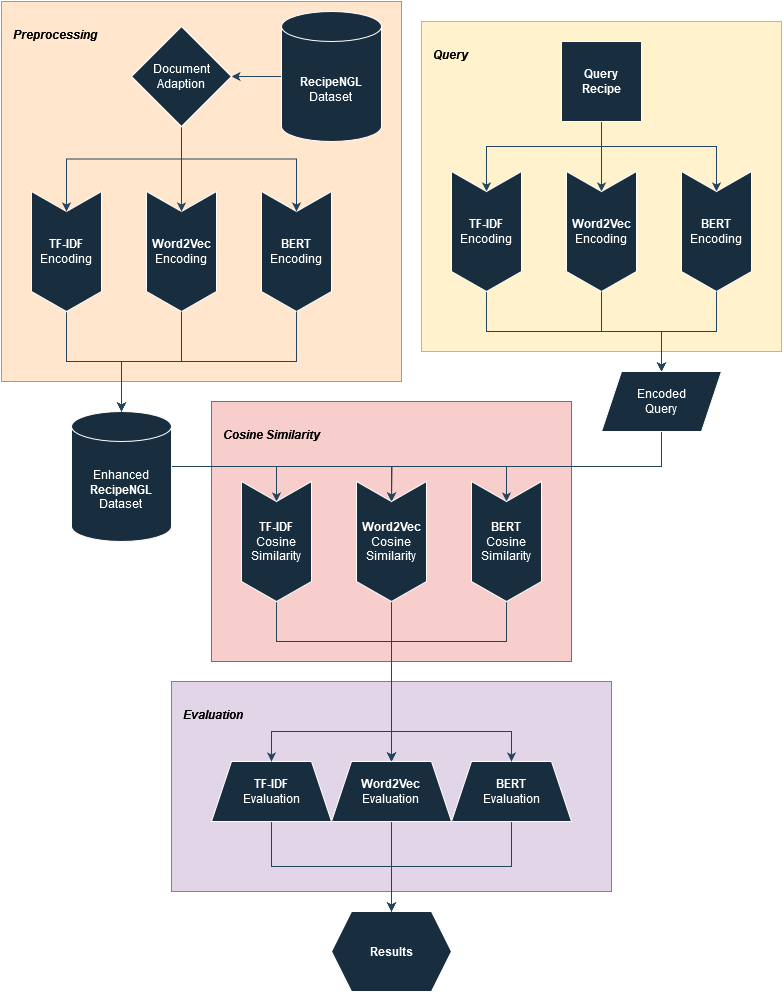
\includegraphics[width=1\linewidth]{graph.png}
    \caption{Shows the pipeline of our AIR project.}
    \label{fig:graph}
\end{figure}

The main tasks of the project are the following:
\begin{itemize}
    \item \textbf{Project Implementation and Experiments.} 
    The project implementation will include pre-processing the dataset, which involves modifying the dataset to include the embeddings created with \wordtovec and the \bert model. 
    Additionally, the \tfidf table has to be computed. \\
    When handling a query, the following steps are required: \\
    Before querying our dataset with the user-provided recipe, we need to extract the \wordtovec and \bert embeddings as well as the \tfidf representation.
    We can then compute the \cossim between the query representation and the entries in the dataset and retrieve a certain number of the most similar recipes for each method.
    These results are displayed to the user. \\
    The retrieved recipes from the different methods will be compared and evaluated in terms of similarity and relevance.
    
    \item \textbf{Report and Presentation.} 
    We will summarize our findings and results in a report and present them in the lecture. 
    We aim to create plots and figures to display the results of our evaluation.
    Additionally, we will propose future work and discuss the limitations of our information retrieval setup.
\end{itemize}


% ---------------------------------------------------------------------------------------------------------------
\section{Dataset and Processing}
To find a proper dataset, we browsed the available datasets on \huggingface.
Specifically, we found a well-populated dataset of recipes with around one million entries: \dataset \cite{bien-etal-2020-recipenlg}. 

To adapt the dataset for our use cases, we will annotate the database with the results of the \tfidf, \wordtovec, and \bert embeddings for the use in \textit{Cosine Similarity} computations.

Since we are not certain if we will be able to handle the full dataset, we might need to adjust the dataset size for the final project.


% ---------------------------------------------------------------------------------------------------------------
\section{Methods and Models}
\begin{itemize}
    \item \textbf{TF-IDF.} 
    We use \tfidf as a traditional information retrieval method and as a baseline for comparison with the advanced information retrieval methods. 
    We create a \tfidf table for our preprocessed dataset and use \cossim to find similar recipes based on our query recipe. 
    \item \textbf{Word2Vec.} 
    We apply \wordtovec to extend the dataset with vector representation embeddings. 
    \item \textbf{Bert-Embeddings.} 
    We use \bert (Bidirectional encoder representations from transformers) to enhance our dataset by representing text as a sequence of vectors using self-supervised learning.
    The model we use is a pre-trained one. 
    We use it to add embeddings to our dataset and computing the \cossim between the query recipe and recipes in the dataset to retrieve the most relevant ones.
    \item \textbf{\cossim.} 
    We use cosine similarity to measure the similarity between recipes across all three types of embeddings. 
    Then, we rank the recipes by similarity and return the most relevant ones to the user.
\end{itemize} 

Our \bert model is also available on \huggingface.
Specifically, we would selected \bertmodel to produce \bert embeddings.
For \tfidf and \wordtovec we will use implementations from existing python libraries.


% ---------------------------------------------------------------------------------------------------------------
\section{Evaluation}
We will individually judge the precision score for the retrieved recipes.
This results in four precision scores per query for each method.
We will take the mean of these scores to arrive at a single score per method per query. 
Furthermore, we will compute an overall mean for each method, resulting in three scores that represent the strength of each method. 
For example, assume we have $n$ query recipes and $k$ persons ranking each result.
Then the overall score $S_m$ for method $m$ would be defined as follows (where $I_{i,j}$ represents the individual precision rating of person $j$ for the given query recipe $i$):
\begin{align*}
    S_m = \frac{1}{n \cdot k} \sum_{i=1}^n \sum_{j=1}^k I_{i, j}
\end{align*}
Finally, we will use these results to address our research questions and compare the different retrieval methods.

% ---------------------------------------------------------------------------------------------------------------
\section{Member Roles}
We plan to distribute the tasks among the members as follows:
\begin{itemize}
    \item \textbf{Markus Auer-Jammerbund:} Report, Query pipeline setup, Evaluation
    \item \textbf{Jonas Pfisterer:} Report, \wordtovec embeddings, Evaluation
    \item \textbf{Thomas Knoll:} Design Document, \bert embeddings, Evaluation
    \item \textbf{Thomas Puchleitner:} Design Document, \tfidf handling, Result processing, Evaluation
\end{itemize}
\clearpage
\bibliographystyle{IEEEtran}
\bibliography{bibliography}

\end{document}
